\section{Methodology}
\label{sec:method}
The following section presents the methodological structure of the research project, driven by the research questions described in section \ref{sec:intro}.\newline
Since trust is a subjective experience (see section \ref{subsec:trust}), it must be evaluated in a user study. For a user study, a use case scenario helps to create a realistic environment and ensure applicability of the results for practitioners. Based on section \ref{sec:background}, the following aspects are required for a use case scenario to answer the research questions:
\begin{enumerate}
	\item \textit{Realistic application scenario} that participants of a user study can relate to and feel into.
	\item \textit{Negative consequences for classification errors}: Possible areas are presented in section \ref{subsubsec:application_areas}, but not all of them are feasible to be investigated in this research project. Data with sensitive content are (fortunately) not freely available, and high-risk domains like criminal justice and terrorism detection enclose their data likewise. Datasets used to gain economic advantage over competitors are often kept confidential or being censored. \cite{diakopoulos2016accountability}.
	\item \textit{Augmented intelligence setting} in which a human collaborates with a machine learning classifier, ensuring that the user's ``willingness to accept a computer-generated recommendation" \cite{vorm2018assessing} is applicable as a proxy measure for trust.
\end{enumerate}
To meet the requirements, we use the scenario of a company's social media channel targetting teenagers and young adults of 15-20 years old. The use case task concerns the identification of offensive texts supported by a machine learning system trained to detect offensiveness. Participants of the study take on the role of a social media moderator and administrator responsible for the content posted within the social media channel. 
\begin{figure} [H]
	\centering
	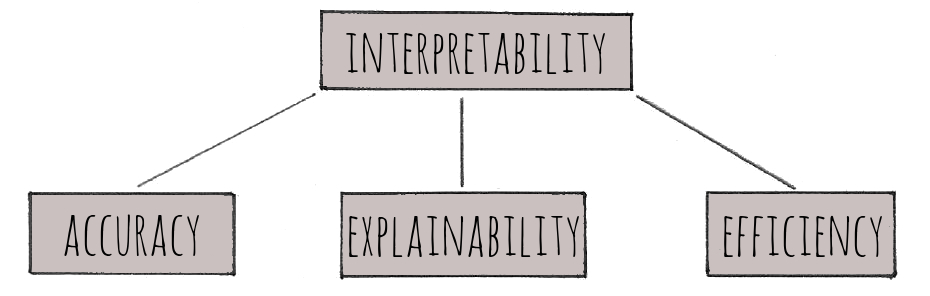
\includegraphics[width=0.7\linewidth]{img/model2}
	\caption{Model of interpretability as defined in \cite{ruping2006learning}}
	\label{fig:model_interpretability}
\end{figure}
\noindent In his model of interpretability, \cite{ruping2006learning} mentions accuracy, explainability, and efficiency as the three main aspects (see figure \ref{fig:model_interpretability}). Interpretability is a positive factor for trust (see section \ref{subsubsec:Explanation Goals}), leading to the assumption that accuracy, explainability, and efficiency have the potential to influence user trust. \textit{Efficiency} relates to the time and mental resources an average user needs to understand the explanation. While efficiency plays a role for user trust, it is not a particular topic in question for this research project. We aim to keep the efficiency constant and minimal throughout our research and therefore adopt the minimum explanation setup suggested by \cite{goodman16eu}: showing how the input features relate to the prediction of a classifier. \newline
\textit{Accuracy} describes the classifier's ability to correctly classify data points (differing from \textit{fidelity}, which describes the explanation's ability to correctly explain the model). To examine the influence of accuracy on user trust, the user's relation with classifiers at varying accuracy levels will be tested. We are especially interested in the extremes as well as a ``realistic" accuracy level in between both extremes and therefore build three systems in total: a very good classifier (0.9 accuracy), a medium classifier (0.7 accuracy), and a bad classifier (0.1 accuracy). We explicitly exclude random classification, since we aim to have a condition in which a meaningful (i.e. truthful) explanation is generated - which is impossible for random class assignment.\newline
Finally, \textit{explainability}, as explained in section \ref{subsec:explainability}, concerns the communication of reasons for an event. For investigating the influence of the explanation's truthfulness, we aim to compare explanations with varying informative content (i.e. varying level of fidelity). The research design is inspired by the copy machine experiment presented in \cite{langer1978mindlessness}, that compared truthful explanations, ``placebic" or dishonest explanations, and a condition without any explanation.



\subsection{Use Case Implications}
The use case scenario takes the user study participants to the topic of offensive language detection for the purpose of youth protection on the internet. \cite{chen2012detecting} define offensive language based on the work of \cite{jay2008pragmatics} as a composition of three categories:
\begin{itemize}
	\item \textit{Hateful language}: language that disparages someone on the basis of a protected trait (e.g. ethnicity, religion, nationality, gender, sexuality, disability, age \cite{diakopoulos2016accountability})
	\item \textit{Pornographic language}: language with explicit sexual content for ``sexual arousal and erotic satisfaction" \cite{chen2012detecting}
	\item \textit{Vulgar language}: language with obscenity and profanity referring to ``sex or bodily functions" \cite{chen2012detecting}	
\end{itemize}
Although offensive language and hate speech are not accurately separated, \cite{davidson2017automated} argues that hate speech is always connected to the expression of hatred, while offensive language uses words that are hate speech in some contexts, but not in others. An example can be found in slang language. The word ``bitch" can be amongst others defamatory, neutral, or an expression of friendship. The ``urban dictionary" lists nine different typical applications\footnote{https://www.urbandictionary.com/define.php?term=bitch}, not all of them being pejorative. In this research project, we adopt the definition of \cite{chen2012detecting} and do not particularly differentiate between hate speech and offensive language to match the use case scenario. Not only hate speech, but also positively meant offensive language should not be broadcasted to a youth audience.\newline
To train machine learning classifiers on offensive language, an annotated dataset is needed. Ideally, the dataset is labelled by human annotators, distinguishes between offensive language and non-offensive language, and contains texts from one or more social media platforms.

\subsubsection{Dataset Selection}
Few datasets with offensive language texts are publicly available. Table \ref{tab:StatsAllDatasets} presents an overview of four available datasets, their sizes and class balances.\newline
\begin{table}[H]
	\centering
	\begin{tabular}{llll}
		\textbf{Corpus} & \textbf{Size} & \textbf{Classes} & \textbf{Split} \\ \midrule
		Davidson\footnotemark[1] & 25,000 & \begin{tabular}[c]{@{}l@{}} hate speech\\offensive\\neither\end{tabular} & \begin{tabular}[c]{@{}l@{}} 6\%\\77\%\\17\%\end{tabular} \\ \midrule
		Imperium\footnotemark[2] & 3,947 & \begin{tabular}[c]{@{}l@{}} neutral\\insulting\end{tabular} & \begin{tabular}[c]{@{}l@{}} 73\%\\27\%\end{tabular} \\ \midrule
		Analytics Vidhya\footnotemark[3] & 31,962 & \begin{tabular}[c]{@{}l@{}} hate speech\\no hate speech\end{tabular} & \begin{tabular}[c]{@{}l@{}} 7\%\\93\%\end{tabular} \\ \midrule
		SwissText\footnotemark[4] & 159,570 & \begin{tabular}[c]{@{}l@{}} toxic\\severe\_toxic\\obscene\\threat\\insult\\hate speech\\neither\end{tabular} & \begin{tabular}[c]{@{}l@{}} 10\%\\1\%\\5\%\\0.3\%\\5\%\\1\%\\72.7\%\end{tabular} \\ \bottomrule        
	\end{tabular}
	\caption{Publicly available datasets for offensive language texts}
	\label{tab:StatsAllDatasets}
\end{table}
\footnotetext[1]{https://github.com/t-davidson/hate-speech-and-offensive-language}
\footnotetext[2]{https://www.kaggle.com/c/detecting-insults-in-social-commentary/data}
\footnotetext[3]{https://datahack.analyticsvidhya.com/contest/practice-problem-twitter-sentiment-analysis/}
\footnotetext[4]{https://www.swisstext.org/workshops/2018/Hackathon.html}
\setcounter{footnote}{4}
\noindent While the dataset of SwissText has the most fine-grained labelling of its data points, details on how the labels were assigned (i.e. number of annotators, inter-annotator agreement score, definition of the classes) are not available. The same holds for the datasets of Analytics Vidhya and Imperium.\newline
In contrast, Davidson's datasets comes with a description of how the data points were collected, how the classes are defined, and uses at least three annotators per text. Furthermore, Davidson's dataset contains the most data points labelled as offensive: roughly 20750 Tweets fall into this category, while the Analytics Vidhya dataset contains 2240 hate speech texts, SwissText 1600, and Imperium 1000.\newline
Throughout the literature, different definitions of hate speech and offensive language are given. For using a dataset in a user study with the scenario of a social media administrator, the definition of the label has to be clear. We therefore choose to work with the dataset of Davidson et al., as it offers the most detailed description of its labels and how the labels were obtained.


\subsubsection{Twitter Data Preprocessing}
\label{subsubsec:tweet_cleaning}
Tweets exhibit some special characteristics. First, the maximum length of a single Tweet is 140 characters. Twitter doubled the length in November 2017, yet the dataset was collected before this data and therefore contains only Tweets of 140 characters or shorter. Twitter users found creative ways to make use of the 140 characters given, leading to the usage of short URLs instead of original URLs \cite{xiang2012detecting}, intentional reductions of words (e.g. ``nite" instead of ``night") \cite{xiang2012detecting}, abbreviations \cite{gupta2018proposed}, emojis \cite{ghorai2016information} \cite{watanabe2018hate} and smilies \cite{smailovic2013predictive} \cite{hovelmann2017fasttext}.\newline
Furthermore, social media content can be unstructured, with word creations that are non in standard dictionaries, like slang words \cite{gupta2018proposed} \cite{watanabe2018hate}, intentional repetitions \cite{xiang2012detecting} \cite{hemalatha2012preprocessing} \cite{montani2018tuwienkbs} \cite{rother2018ulmfit} (e.g. ``hhheeeey"), contractions of words \cite{smailovic2013predictive} \cite{hemalatha2012preprocessing}, and spelling mistakes. Although those new word formations do not appear in the dictionary, they are ``intuitive and popular in social media" \cite{hu2012text}. \newline
On Twitter, it is custom to mention other users within a Tweet by adding ``@"+username \cite{xiang2012detecting} \cite{montani2018tuwienkbs} \cite{watanabe2018hate} \cite{rother2018ulmfit}, retweeting (i.e. answering to) a Tweet \cite{xiang2012detecting} \cite{hemalatha2012preprocessing}, and summarizing a Tweet's topic with ``\#"+topic \cite{xiang2012detecting} \cite{watanabe2018hate}. \newline
Other problems in text mining are the handling of stop words \cite{xiang2012detecting} \cite{ghorai2016information} \cite{gupta2018proposed}, language detection \cite{xiang2012detecting}, punctuation \cite{ghorai2016information} \cite{hemalatha2012preprocessing} \cite{montani2018tuwienkbs}, negation \cite{watanabe2018hate}, and case folding \cite{ghorai2016information} \cite{gupta2018proposed} \cite{rother2018ulmfit}.\newline
Researchers have developed different strategies for preprocessing Tweets. One possible approach is to simply remove URLs, username, hashtags, emoticons, stop words, or punctuation \cite{xiang2012detecting} \cite{ghorai2016information} \cite{hemalatha2012preprocessing} \cite{montani2018tuwienkbs} \cite{gupta2018proposed} \cite{watanabe2018hate}. A reason to eliminate those tokens can be that they assumably do not hold information relevant to the classification goal \cite{hemalatha2012preprocessing}. Words that only exist for syntactic reasons (this concerns primarily stop words) can be omitted when focussing on sentiment or other semantic characteristics \cite{ghorai2016information}. Mentions of other users are likewise not informative for sentiment analysis and are often removed from the texts \cite{xiang2012detecting} \cite{watanabe2018hate}. Depending on the dataset size, normalising the texts strongly by removing punctuation and emojis, as well as lowercasing the texts, can decrease the vocabulary size \cite{ghorai2016information}. Especially on Twitter with its restricted text size, users tend to use shortened URLs. Short URLs have a concise, but often cryptic form, and redirect to the website with the original, long URL. While website links can encode some information on a topic, this information is lost when using a shortened URL. Removing the shortened URLs without replacement can be a step in preprocessing Tweets \cite{xiang2012detecting}.\newline
Rather than removing tokens, they can also be replaced by a signifier token, e.g. a complete link by ``$<<<$hyperlink$>>>$" \cite{hovelmann2017fasttext}. In Tweets, such signifier tokens are used for mentions of usernames \cite{smailovic2013predictive} \cite{hovelmann2017fasttext} \cite{rother2018ulmfit}, URLs \cite{smailovic2013predictive} \cite{hovelmann2017fasttext} \cite{rother2018ulmfit}, smilies \cite{hovelmann2017fasttext} or negations \cite{smailovic2013predictive}. Using signifier tokens eliminates some information, i.e. which user was mentioned or which website was linked, but retains the information that a mention or link exists. Tokens can also be grouped by using signifier tokens, i.e. tokens with similar content are summarised with a single token. \cite{hovelmann2017fasttext} uses this technique to group smilies with similar sentiment and Twitter usernames related to the same company.\newline 
Case folding is often addressed by converting Tweets to lower case \cite{ghorai2016information} \cite{hovelmann2017fasttext} \cite{gupta2018proposed}.\newline

\subsubsection{Offensive Language Detection}
\label{subsubsec:method_classifier}
Offensive language and hate speech detection systems noted in related literature use a wide range of classifiers.\newline
The data engineers of the dataset we chose tested a variety of classifiers for distinguishing hate speech, offensive language, and non-offensive language \cite{davidson2017automated}. The best results were found for a logistic regression system and a linear support vector machine (SVM), reaching a better performance than Naive Bayes, decision tree, and random forests. They eventually use logistic regression because it offers continuous output and showed promising performance in similar applications. \cite{montani2018tuwienkbs} use an ensemble setting with a logistic regression classifier and a random forests system to generate features that are subsequently forwarded to a final logistic regression classifier. Recurrent neural networks (RNN), a type of neural networks, was also used for hate speech detection \cite{del2017hate, rother2018ulmfit}. \cite{del2017hate} compare a RNN and an SVM and found out that the SVM performs better on detecting hate speech, while both classifiers show equal performance for classifying texts without hate speech. Using only a dictionary to filter out offensive words is not a sufficient solution for offensive language detection. Implicit offensiveness describes texts that have an offensive meaning, yet do not contain any words registered in a hate speech database. \cite{klenner2018offensive} focus on implicit offensiveness. They examine each word in a text individually, and then determine the class for a text by counting the number of offensive words divided by the total amount of words. For texts encoded in a vector space model (using e.g. fasttext or word2vec), \cite{gupta2018proposed} suggest using cosine similarity measured on a scale of 0.0-1.0 with the class boundary at 0.6. Although not focussing on offensive language in particular, but on general sentiment of texts, \cite{chen2018learning} developed a system architecture called ``Learning to Explain" (L2X) that uses a convolutional neural network (CNN) to classify. In a second step, the algorithm determines the $k$ most decisive words in the input text using mutual information analysis. \medskip \newline
Our goal are three systems with accuracies of 0.9, 0.7, and 0.1, which hold the potential to create truthful explanations for the decision process. We therefore choose L2X for the very good classifier, and use its inverted version (the same setup but trained on inversely labelled training set) for the bad classifier. We then use a time-tested classifier with average results: logistic regression. The advantage of logistic regression for our purpose is that if offers the coefficients for all input features which helps to generate explanations. 

\subsubsection{Explanations}
\label{subsubsec:method_explanations}
To answer the research questions \textbf{RQ 2} and \textbf{RQ 3}, the level of truthfulness, i.e. fidelity, needs to be varied. Following the setup of \cite{langer1978mindlessness} in the copy machine experiment, we aim to generate three types of explanations: (1) a good explanation with high fidelity to the underlying model, (2) a bad explanation with placebic, i.e. nonsensical information, and (3) an ``explanation" with zero explanatory content.\newline
For generating explanations, we focus on input features and their decisive power regarding the classification result, as suggested in the minimum explanation setup by \cite{goodman16eu}. Our dataset contains Tweets, hence textual input, encoded with the bag-of-words method. The individual words in a text are therefore the input features. Showing how the words relate to the prediction can be done via highlighting (\cite{arras2017relevant, chen2012detecting, feng2018pathologies}).\newline
The three explanation types will be generated as follows:
\paragraph{Good explanations}
All three classifiers (L2X, Inverse L2X, and logistic regression) are able to give information about which of the input features are most decisive for the classification result. The L2X algorithm is especially made to select most decisive features - in this case single words within a text -, while logistic regression offers information about the coefficients, which are equal to the influence of individual features on the classification result. For both algorithms, the decisive words in a text can therefore be determined and subsequently communicated to the user by highlighting.
\paragraph{Bad explanations}
Similar to the ``placebic" explanations used in the copy machine experiment \cite{langer1978mindlessness}, the bad explanations in this research project do not provide useful information. They are, on the surface, visually similar to good explanations, but without being truthful to the underlying model. To generate nonsensical explanations, we randomly draw words from the texts. By using random selection, we assure that no human-readable pattern shows in the bad explanations.
\paragraph{Zero explanations}
The opposite of good explanations with high informative content is zero information content, thus no explanation at all. It needs to be noted that the explanation is not tied to the classification result (the label). The system can show no explanation but still show the decision. 



\subsection{User Study}
Trust and perceived understanding are subjective experiences and hence must be evaluated with a user study. We therefore aim to answer the research questions in a user study with tasks of the use case scenario explained above. Participants of the study should take the role of a social media administrator. As trust builds up over time and is build on repeated experiences with an agent \cite{rempel1985trust}, participants of the user study need to have repeated interaction with the system. We therefore show them a set of Tweets combined with the classifier's decision and explanation. The study is designed and run on the \textit{SoSci Survey}\footnote{https://www.soscisurvey.de/en/index} platform.\newline

\subsubsection{Conditions}
Explainability and accuracy are the two variables in question for the study. Based on the copy machine experiment \cite{langer1978mindlessness}, three explanation types are generated: (1) no explanation, (2) a placebic explanation, and (3) an informative explanation. We want to test the influence of accuracy on trust with three classifiers: (1) very good with 0.9 accuracy level, (2) medium at 0.7 accuracy, and (3) bad with 0.1 accuracy. Evaluating each classifier-explanation combination leads to 9 conditions that we encode as follows:
\begin{table}[H]
	\centering
	\begin{tabular}{l}
		\textbf{Condition}\\ \midrule
		super-good\\
		super-rand\\
		super-no\\
		medium-good\\
		medium-rand\\
		medium-no\\
		bad-good\\
		bad-rand\\
		bad-no\\ \bottomrule
	\end{tabular}
	\caption{List of classifier-explanation combinations evaluated in the user study}
	\label{tab:conditions}
\end{table} 

\subsubsection{Measures}
Perceived understanding can be evaluated with a self-assessment questionnaire.\newline
For measuring trust in the automatic decision system, we use the trust questionnaire for automtated systems by \cite{ruping2006learning}. However, \cite{langer1978mindlessness} observed the ignorance of informational content in explanations only in a ``mindless", i.e. inattentive state. We therefore use a second measure of trust, the proxy measure of willingness to adopt a classifier's recommendation. The proxy can be measured by exposing the participants to the Tweets once without the system and a second time with the system and observe the changes in classification that were made. A detailed list of all questions used in the survey can be found in appendix {\color{red}X}.

\subsubsection{Procedure}
On both platforms, the participants receive a link to the survey. As soon as the participant opens the survey URL, the survey starts. The survey consists of the following content:
\begin{enumerate}
	\item Introduction \& consent form
	\item \textit{Scenario 1}: Social media administrator and manual offensive language detection
	\item \textit{Tweet block 1}: 15 Tweets for classification, on individual pages (no system)
	\item \textit{Scenario 2}: Introduction to automatic decision system supporting the task
	\item \textit{Tweet block 2}: Repetition of 15 Tweets for classification, on individual pages (with system)
	\item Perceived understanding \& trust questionnaire
	\item Demographics
	\item Outroduction \& crowdsourcing completion codes
\end{enumerate}
In general, the study contains three blocks plus an introduction and outroduction section. The first block treats a scenario in which the participant plays the role of a ``social media administrator" of a company with a young target group (15-20 years old). The task of the social media administrator is to identify content with offensive language in order to block such comments or Tweets. The next 15 pages of the survey contain one Tweet each, shown on a screenshot of a management tool, and ask the participant to classify the text as offensive or not offensive as shown in figure. The order in which the Tweets are shown is randomised for each participant. There are 10 different sets of Tweets available (without overlap), to avoid effects from the specific wording or topics in the small set of 15 Tweets. At the start of the survey, each participant is randomly assigned to one Tweet set by the system.\newline
The second block introduces the automatic decision system. The participant is again asked to classify 15 ``very similar" Tweets, which are, in fact, identical to the ones shown in the first block. This particular formulation aims to liberate the participants from the urge to classify each text with exactly the same label as in the first block. The ordering of the Tweets is random and hence very likely to be different from the ordering of the first block. In total, 9 conditions exist: three systems with each three explanation types (informative, placebic, no explanation) each. Each participant has one condition assigned at the beginning of the survey, such that there is an equal distribution of conditions in finished questionnaires. \newline
Finally, the last block contains three questions regarding perceived understanding, 19 items measuring the user's trust including an attention check, and 5 demographic questions (gender, age, country, ethnicity, English language level).\newline

\subsubsection{Analysis}
The between-subject setup described in the previous paragraph is tested in a pilot study with 11 participants. The participants are recruited via ``Prolific" and receive a compensation of 2.00 GBP (2.28 EUR). They complete the study in ``pretest" mode, which shows an additional comment box at the bottom of each survey page.\newline
The main study is set up as a quantitative study without open questions or free text input. Basic frequency analysis is used for the demographic items in order to understand the background of the participants. Three topics are investigated in a statistical manner: perceived understanding (3 items), self-reported trust (19 items), and observed trust via proxy. For the first two, a 5-point Likert scale is employed.\newline
A \textit{Perceived understanding} score is calculated for each participant by taking the mean of the ratings for all three items in the questionnaire. The trust questionnaire used to measure \textit{self-reported trust} contains 14 positive items and 5 inverse items. A single mean score is calculated by taking the average over the positive items and the maximum rating minus the mean of the inverse items. As a second trust measure, \textit{observed trust} is investigated via the proxy of willingness to follow a system's recommendation. The survey contains a block of manual classification without the system, and a second round with the information provided by the automated decision system. In each block, participants classify the same set of Tweets. We can therefore determine how often a participant switches his or her classification out of 15 possible cases, and how often the change is made in agreement with the classifier's prediction but against the truth. Since the three classifiers offer different amount of opportunities to change with the classifier's prediction away from the truth (maximum 14 cases for the bad classifier as opposed to maximum 1 case for the very good classifier), the proxy measure is calculated and normalised as follows for each participant:
\[ \frac{changes\_towards\_prediction\_against\_truth}{opportunities\_for\_change\_against\_truth} \]
Cases in which the very good classifier does not make any misclassification (hence no opportunity for the user to change in favour of the classifier and in contradiction to the truth) are excluded, because no valid conclusion can be drawn from these cases.\newline
The goal of the statistical analysis for all three topics (perceived understanding, self-reported trust, observed trust via proxy) is to identify differences between different conditions. To determine whether the samples are normally distributed, we use the Shapiro-Wilk test \footnote{https://docs.scipy.org/doc/scipy/reference/generated/scipy.stats.shapiro.html} for normality from the SciPy library). We use the Mann-Whitney U test to compare two samples, since it does not assume normal distribution nor equal sample sizes or variances. For sample sizes above 20 data points, we employ SciPy's approximation\footnote{https://docs.scipy.org/doc/scipy/reference/generated/scipy.stats.mannwhitneyu.html} of the Mann-Whitney U test. In case of smaller sample sizes, we use the exact implementation\footnote{https://mail.python.org/pipermail/scipy-dev/2015-March/020475.html} of the Mann-Whitney U test as described in \cite{cheung1997mann}.

\subsubsection{Apparatus}
The user study is set up as an online study, the study can therefore be taken at a self-chosen location on private devices. Participants are asked to completed the survey on a notebook, desktop computer or tablet. For consistency with the use case scenario, screenshots of a fictive social media management platform show the input texts, decisions and explanations. The screenshots have a ratio of 900px (width) to 253px (height). To ensure that improper scaling of the screenshots does not influence the participants' perception, devices with small screens (e.g. smartphones and other mobile devices) are excluded. However, which device participants finally use cannot be verified. No further requirements are made regarding the equipment of the participant's device.

\subsubsection{Participants}
Participants are recruited via the paid science crowdsourcing platform ``Prolific"\footnote{https://prolific.ac} and ``SurveyCircle"\footnote{https://www.surveycircle.com}, an unpaid participant recruitment platform based on mutuality. All participants recruited on the paid platform ``Prolific" receive a compensation of 1.40 GBP (1.60 EUR) for an estimated expenditure of time of 12 minutes. Participants from ``SurveyCircle" receive a reward of 4.4 Study Points. On both platforms, individuals younger than 18 years are excluded to participate for reasons of consent by a major. The use case scenario includes reading and understanding real-life Tweets with slang words, grammatical and literal errors. The platforms therefore screen for people being fluent in English. The study questionnaire includes an attention check question, asking the participants to answer ``completely disagree" in between the trust questionnaire items assessed on a 5-point Likert scale. Data from participants who fail to answer the attention check correctly is excluded from the analysis. Furthermore, only complete responses are analysed, i.e. data from participants who reach the last page of the survey.








